% RAG Pipeline Presentation
% Author: Mondweep Chakravorty
% Date: December 2025
% Knowledge Sharing Session

\documentclass[aspectratio=169]{beamer}

% Theme and styling
\usetheme{Madrid}
\usecolortheme{whale}
\setbeamertemplate{navigation symbols}{}
\setbeamertemplate{footline}[frame number]

% Packages
\usepackage{tikz}
\usepackage{listings}
\usepackage{xcolor}
\usepackage{fontawesome5}
\usepackage{tcolorbox}

% Custom colours
\definecolor{ragblue}{RGB}{0,212,255}
\definecolor{ragpurple}{RGB}{124,58,237}
\definecolor{codebg}{RGB}{40,44,52}
\definecolor{codegreen}{RGB}{152,195,121}
\definecolor{codeyellow}{RGB}{229,192,123}

% Code listing style
\lstdefinestyle{pythonstyle}{
    backgroundcolor=\color{codebg},
    basicstyle=\ttfamily\scriptsize\color{white},
    keywordstyle=\color{ragpurple},
    stringstyle=\color{codegreen},
    commentstyle=\color{gray},
    breaklines=true,
    frame=single,
    rulecolor=\color{ragblue},
    numbers=left,
    numberstyle=\tiny\color{gray},
    showstringspaces=false
}

% Title information
\title[RAG Pipeline]{\textbf{Building a RAG Pipeline}}
\subtitle{Using LangChain and FAISS}
\author{Mondweep Chakravorty}
\institute{Knowledge Sharing Session}
\date{December 2025}

\begin{document}

% Title slide
\begin{frame}
    \titlepage
\end{frame}

% Agenda
\begin{frame}{Session Agenda}
    \begin{columns}
        \begin{column}{0.5\textwidth}
            \begin{itemize}
                \item[\faIcon{clock}] \textbf{2 mins} - Introduction
                \item[\faIcon{chalkboard-teacher}] \textbf{5 mins} - Presentation
                \item[\faIcon{code}] \textbf{3 mins} - Code Demo
                \item[\faIcon{comments}] \textbf{30 mins} - Q\&A
            \end{itemize}
        \end{column}
        \begin{column}{0.5\textwidth}
            \begin{tcolorbox}[colback=ragblue!10, colframe=ragblue, title=Target Audience]
                Beginners with limited understanding of Generative AI
            \end{tcolorbox}
        \end{column}
    \end{columns}
\end{frame}

% What is RAG?
\begin{frame}{What is RAG?}
    \begin{center}
        \Huge\textbf{\textcolor{ragblue}{R}etrieval \textcolor{ragpurple}{A}ugmented \textcolor{ragblue}{G}eneration}
    \end{center}

    \vspace{1em}

    \begin{tcolorbox}[colback=ragpurple!10, colframe=ragpurple]
        A technique that enhances LLMs by giving them access to external knowledge sources
    \end{tcolorbox}

    \vspace{1em}

    \textbf{The Problem RAG Solves:}
    \begin{itemize}
        \item[\faIcon{calendar-times}] LLMs have knowledge cutoff dates
        \item[\faIcon{ghost}] They can ``hallucinate'' (make things up)
        \item[\faIcon{lock}] They don't know your private/company data
    \end{itemize}
\end{frame}

% RAG vs Standard LLM
\begin{frame}{RAG vs Standard LLM}
    \begin{columns}
        \begin{column}{0.48\textwidth}
            \begin{tcolorbox}[colback=red!10, colframe=red!70, title=\faIcon{times-circle} Without RAG]
                \textbf{User:} ``What is our company's leave policy?''

                \vspace{0.5em}

                \textbf{LLM:} ``I don't have information about your specific company policies...''
            \end{tcolorbox}
        \end{column}
        \begin{column}{0.48\textwidth}
            \begin{tcolorbox}[colback=green!10, colframe=green!70, title=\faIcon{check-circle} With RAG]
                \textbf{User:} ``What is our company's leave policy?''

                \vspace{0.5em}

                \textbf{RAG:} ``Your company offers 25 days annual leave per year...''
            \end{tcolorbox}
        \end{column}
    \end{columns}
\end{frame}

% How RAG Works - Diagram
\begin{frame}{How RAG Works}
    \begin{center}
        \begin{tikzpicture}[
            node distance=1.5cm,
            box/.style={rectangle, draw=ragblue, fill=ragblue!20, rounded corners, minimum width=2.5cm, minimum height=1cm, align=center, font=\small},
            arrow/.style={->, thick, ragpurple}
        ]
            % Nodes
            \node[box] (question) {\faIcon{question-circle} Question};
            \node[box, right of=question, xshift=2cm] (embed) {\faIcon{vector-square} Embed Query};
            \node[box, right of=embed, xshift=2cm] (search) {\faIcon{search} Search Docs};
            \node[box, right of=search, xshift=2cm] (generate) {\faIcon{robot} Generate};
            \node[box, below of=search, yshift=-0.5cm] (vectordb) {\faIcon{database} Vector DB\\(FAISS)};
            \node[box, below of=vectordb, yshift=-0.5cm] (docs) {\faIcon{file-alt} Your\\Documents};

            % Arrows
            \draw[arrow] (question) -- (embed);
            \draw[arrow] (embed) -- (search);
            \draw[arrow] (search) -- (generate);
            \draw[arrow] (docs) -- (vectordb);
            \draw[arrow] (vectordb) -- (search);

            % Answer
            \node[box, fill=green!20, draw=green!70, right of=generate, xshift=2cm] (answer) {\faIcon{check} Answer};
            \draw[arrow, green!70] (generate) -- (answer);
        \end{tikzpicture}
    \end{center}
\end{frame}

% Key Components
\begin{frame}{Key Components}
    \begin{table}
        \centering
        \begin{tabular}{|l|l|l|}
            \hline
            \textbf{Component} & \textbf{Purpose} & \textbf{Tool} \\
            \hline
            Document Loader & Load your files & LangChain \\
            \hline
            Text Splitter & Break into chunks & LangChain \\
            \hline
            Embeddings & Convert text $\rightarrow$ vectors & OpenAI \\
            \hline
            Vector Store & Store \& search vectors & FAISS \\
            \hline
            LLM & Generate answers & OpenAI GPT \\
            \hline
            Chain & Connect it all & LangChain \\
            \hline
        \end{tabular}
    \end{table}
\end{frame}

% What are Embeddings?
\begin{frame}{What are Embeddings?}
    \begin{tcolorbox}[colback=ragblue!10, colframe=ragblue, title=Embeddings = Numbers that capture meaning]
        \begin{verbatim}
"King"  → [0.2, 0.8, 0.1, ...]
"Queen" → [0.3, 0.7, 0.1, ...]  ← Similar vectors!
"Car"   → [0.9, 0.1, 0.5, ...]  ← Different vector
        \end{verbatim}
    \end{tcolorbox}

    \vspace{1em}

    \begin{center}
        \Large Similar concepts have similar vectors = \textbf{\textcolor{ragpurple}{Semantic Search}}
    \end{center}
\end{frame}

% What is FAISS?
\begin{frame}{What is FAISS?}
    \begin{center}
        \Huge\textbf{FAISS}

        \large Facebook AI Similarity Search
    \end{center}

    \vspace{1em}

    \begin{itemize}
        \item[\faIcon{facebook}] Open-source library from Meta
        \item[\faIcon{database}] Efficiently stores millions of vectors
        \item[\faIcon{bolt}] Finds similar vectors incredibly fast
        \item[\faIcon{pound-sign}] Free to use (no API costs!)
    \end{itemize}
\end{frame}

% RAG Pipeline Steps
\begin{frame}{The RAG Pipeline in 5 Steps}
    \begin{enumerate}
        \item[\textcolor{ragblue}{\textbf{1}}] \textbf{LOAD} $\rightarrow$ Get your documents
        \item[\textcolor{ragblue}{\textbf{2}}] \textbf{SPLIT} $\rightarrow$ Break into chunks
        \item[\textcolor{ragblue}{\textbf{3}}] \textbf{EMBED} $\rightarrow$ Convert to vectors
        \item[\textcolor{ragblue}{\textbf{4}}] \textbf{STORE} $\rightarrow$ Save in FAISS
        \item[\textcolor{ragblue}{\textbf{5}}] \textbf{QUERY} $\rightarrow$ Retrieve + Generate
    \end{enumerate}
\end{frame}

% Code Demo
\begin{frame}[fragile]{Code Demo: Simple RAG Pipeline}
    \begin{lstlisting}[style=pythonstyle, language=Python]
from langchain_community.document_loaders import TextLoader
from langchain_text_splitters import CharacterTextSplitter
from langchain_openai import OpenAIEmbeddings, ChatOpenAI
from langchain_community.vectorstores import FAISS

# 1. LOAD documents
loader = TextLoader("company_policies.txt")
documents = loader.load()

# 2. SPLIT into chunks
splitter = CharacterTextSplitter(chunk_size=500)
chunks = splitter.split_documents(documents)

# 3. EMBED and STORE in FAISS
embeddings = OpenAIEmbeddings()
vector_store = FAISS.from_documents(chunks, embeddings)

# 4. QUERY - retrieve relevant chunks
retriever = vector_store.as_retriever()
docs = retriever.get_relevant_documents("annual leave?")
    \end{lstlisting}
\end{frame}

% Test Results
\begin{frame}{Demo Results}
    \begin{tcolorbox}[colback=codebg, colframe=ragblue, title=\textcolor{white}{Test Output}]
        \textcolor{white}{\textbf{Q: What is the annual leave policy?}}

        \vspace{0.5em}

        \textcolor{codegreen}{A: All full-time employees are entitled to 25 days of annual leave per calendar year. Part-time employees receive a pro-rata entitlement...}

        \vspace{1em}

        \textcolor{white}{\textbf{Q: What are the core working hours?}}

        \vspace{0.5em}

        \textcolor{codegreen}{A: The core working hours are 10:00 AM to 4:00 PM.}
    \end{tcolorbox}
\end{frame}

% Use Cases
\begin{frame}{Use Cases}
    \begin{columns}
        \begin{column}{0.5\textwidth}
            \begin{itemize}
                \item[\faIcon{headset}] \textbf{Customer Support}\\Answer questions from knowledge base
                \item[\faIcon{balance-scale}] \textbf{Legal}\\Search through contracts
                \item[\faIcon{users}] \textbf{HR}\\Query company procedures
            \end{itemize}
        \end{column}
        \begin{column}{0.5\textwidth}
            \begin{itemize}
                \item[\faIcon{flask}] \textbf{Research}\\Explore academic papers
                \item[\faIcon{book}] \textbf{Documentation}\\Chat with your codebase
                \item[\faIcon{hospital}] \textbf{Healthcare}\\Medical knowledge retrieval
            \end{itemize}
        \end{column}
    \end{columns}
\end{frame}

% Key Takeaways
\begin{frame}{Key Takeaways}
    \begin{itemize}
        \item[\textcolor{green}{\faIcon{check}}] \textbf{RAG} = Retrieval + Generation
        \item[\textcolor{green}{\faIcon{check}}] Solves LLM limitations (hallucination, knowledge cutoff)
        \item[\textcolor{green}{\faIcon{check}}] \textbf{LangChain} makes it easy to build
        \item[\textcolor{green}{\faIcon{check}}] \textbf{FAISS} provides free, fast vector search
        \item[\textcolor{green}{\faIcon{check}}] You can build one in \textasciitilde15 lines of code!
    \end{itemize}

    \vspace{1em}

    \begin{tcolorbox}[colback=ragpurple!10, colframe=ragpurple]
        \centering
        \textbf{Try the live demo:} Your Netlify URL here
    \end{tcolorbox}
\end{frame}

% Questions
\begin{frame}{Questions?}
    \begin{center}
        \Huge\faIcon{comments}

        \vspace{1em}

        \Large\textbf{Q\&A Time: 30 minutes}
    \end{center}

    \vspace{2em}

    \textbf{Resources:}
    \begin{itemize}
        \item[\faIcon{globe}] LangChain: \texttt{langchain.com}
        \item[\faIcon{github}] FAISS: \texttt{github.com/facebookresearch/faiss}
        \item[\faIcon{robot}] OpenAI: \texttt{platform.openai.com}
    \end{itemize}
\end{frame}

% Thank you
\begin{frame}
    \begin{center}
        \Huge\textbf{Thank You!}

        \vspace{1em}

        \Large Mondweep Chakravorty

        \vspace{2em}

        \normalsize
        \faIcon{github} github.com/mondweep/vibe-cast
    \end{center}
\end{frame}

\end{document}
